\documentclass[conference]{IEEEtran}
\IEEEoverridecommandlockouts
\usepackage{iftex}
\ifXeTeX
  \usepackage{fontspec}
  \setmainfont{texgyretermes-regular.otf}[BoldFont=texgyretermes-bold.otf,ItalicFont=texgyretermes-italic.otf,BoldItalicFont=texgyretermes-bolditalic.otf]  % Times clone with bold/italic (pdfLaTeX uses IEEEtran's Times instead)
\fi
\usepackage{cite}
\usepackage{amsmath,amssymb}
\usepackage{graphicx}
\usepackage{booktabs}
\usepackage{array}
\usepackage{textcomp}
\usepackage{xcolor}
\usepackage[hidelinks]{hyperref}
\def\BibTeX{{\rm B\kern-.05em{\sc i\kern-.025em b}\kern-.08em T\kern-.1667em\lower.7ex\hbox{E}\kern-.125em X}}

\begin{document}

\title{Social DNA: Community Discovery, Interest Profiling and Verified LLM Explanations on the LastFM Asia Social Network}

\author{\IEEEauthorblockN{{[}Author Name{]}}
\IEEEauthorblockA{\textit{{[}Department, University{]}} \\
{[}City, Country{]} \\
{[}email address{]}}}

\maketitle

\begin{abstract}
Community detection is routinely reported through modularity and partition-similarity scores, but the results are rarely turned into explanations that a non-specialist can audit. This paper presents Social DNA, an end-to-end, reproducible system that (i) detects communities in a social network, (ii) profiles what their members have in common and what distinguishes them, (iii) identifies hub and bridge users, and (iv) exposes all of this through a natural-language analyst in which a large language model (LLM) only \emph{explains} verified, pre-computed results. We apply it to the public LastFM Asia network (7{,}624 users, 27{,}806 mutual-follower edges, 7{,}842 anonymised liked-artist features). Louvain finds 31 communities (modularity $Q=0.8155$) with high stability across 10 random seeds (mean pairwise NMI 0.900) and substantial agreement with greedy modularity optimisation (NMI 0.819). Community interest profiles built from frequency, lift and TF-IDF cosine similarity show that members share only moderate taste internally (mean within-community cosine 0.123), while a few community pairs are very similar (cosine up to 0.880). A hub (degree 216) and a bridge user (degree 62, friends in 13 communities) are shown to be different people. On a fixed 29-question benchmark whose expected values are recomputed from the database, a live Gemini-based analyst reached 95.7\% routing accuracy, 96.7\% numerical correctness and an unsupported-claim rate of 0.1\%, while a deterministic router reached 100\%. Because the dataset has no ground-truth communities, we report consistency measures rather than classification accuracy, and we disclose a post-hoc scorer revision and the limits of a small benchmark.
\end{abstract}

\begin{IEEEkeywords}
community detection, Louvain algorithm, modularity, social network analysis, TF-IDF, large language models, grounded generation
\end{IEEEkeywords}

\section{Introduction}
Online social networks are naturally organised into groups of densely connected users. Finding these groups, understanding what the members share, and identifying the users who link different groups are core tasks in social network analysis \cite{fortunato2010}. In practice the output of a community-detection algorithm is a partition and a modularity score \cite{newman2006}; explaining \emph{why} a group exists or how groups differ is left to the analyst. Large language models can write fluent explanations, but they are prone to hallucination \cite{ji2023}, which is unacceptable when the explanation is supposed to report measured values.

This paper describes Social DNA, a system built around one rule: \emph{every number shown to the user is calculated from the dataset, and the LLM never calculates or chooses data}. The LLM is the last stage of a pipeline and is restricted to paraphrasing verified JSON produced by validated backend functions. Our contributions are:
\begin{enumerate}
\item A reproducible pipeline (acquisition, validation, graph construction, Louvain and greedy-modularity detection, persistence in SQLite) with explicit stability and agreement evaluation that avoids misusing metadata as ground truth.
\item An interest-profiling method for binary attributed users that combines frequency, prevalence and lift with a distinctiveness score, and TF-IDF cosine and Jaccard similarity, including an exact identity for within-community cosine that avoids quadratic computation.
\item A hub-versus-bridge analysis combining sampled betweenness with the participation coefficient.
\item A grounded LLM analyst: function-calling router, parameter validation, refusal of unsupported questions, graceful degradation, and an evaluation protocol with numerical-correctness and unsupported-claim metrics, reported honestly including a scorer revision.
\end{enumerate}
The system is released as open-source Python code with 76 automated tests.

The remainder of the paper reviews related work (Section~\ref{sec:related}), describes the dataset (Section~\ref{sec:data}) and methods (Section~\ref{sec:method}), reports results (Section~\ref{sec:results}), and discusses limitations and future work (Sections~\ref{sec:disc}--\ref{sec:conc}).

\section{Related Work}\label{sec:related}
\textbf{Community detection.} Modularity \cite{newman2006} measures how much denser the links inside groups are than expected under a degree-preserving random model. Greedy agglomerative optimisation was proposed for very large networks by Clauset et al.\ \cite{clauset2004}, and the Louvain method \cite{blondel2008} alternates local node moves with community aggregation and became a standard because of its speed. Louvain can produce badly connected communities, which motivated Leiden \cite{traag2019}; modularity optimisation also has a resolution limit \cite{fortunato2007}. Fortunato's survey \cite{fortunato2010} gives a broad overview. Partitions are commonly compared with normalised mutual information \cite{danon2005} and the adjusted Rand index \cite{hubert1985}; these require a reference partition, which many real networks lack.

\textbf{Attributes and interests.} Attributed-graph clustering combines structure and node attributes \cite{bothorel2015}. Homophily---the tendency of similar people to connect---is a well-documented property of social ties \cite{mcpherson2001}. We follow the classical information-retrieval treatment of sparse feature vectors: TF-IDF weighting \cite{salton1988} and Jaccard overlap \cite{jaccard1901}.

\textbf{Influence and bridges.} Betweenness centrality \cite{freeman1977} identifies users on many shortest paths and can be estimated from sampled sources \cite{brandes2007}; PageRank \cite{page1999} rewards links from well-linked users; the participation coefficient \cite{guimera2005} quantifies how evenly a node's links are spread over communities. The importance of weak ties between groups goes back to Granovetter \cite{granovetter1973}.

\textbf{Grounded LLMs.} Retrieval-augmented generation conditions an LLM on external evidence \cite{lewis2020}, and tool-use approaches let a model call external functions \cite{schick2023}. Our analyst follows this idea in a deliberately strict form: the model selects a function, the backend validates and executes it, and the model only verbalises the returned JSON. We use the Gemini family of models \cite{gemini2023}.

\section{Dataset}\label{sec:data}
We use the LastFM Asia Social Network released with the FEATHER project \cite{rozemberczki2020}, collected from the public LastFM API in March 2020. Nodes are users from Asian countries, undirected edges are mutual follower relations, and each user has a list of liked artists encoded as anonymous feature identifiers. A target file contains an anonymised country code per user. The application downloads the official archive on first launch, validates it, and caches processed files; it does not download it again afterwards.

\begin{table}[t]
\caption{Dataset and network statistics (computed by the validation and metrics modules)}
\label{tab:data}
\centering
\begin{tabular}{lr}
\toprule
Users (nodes) & 7{,}624 \\
Friendships (edges) & 27{,}806 \\
Distinct artist features & 7{,}842 \\
Mean features per user & 395 \\
Users with no features & 173 \\
Duplicate edges / self-loops / isolates & 0 / 0 / 0 \\
Connected components & 1 \\
Density & 0.0010 \\
Mean / median / max degree & 7.29 / 4 / 216 \\
Average clustering coefficient & 0.219 \\
Transitivity & 0.179 \\
\bottomrule
\end{tabular}
\end{table}

Table~\ref{tab:data} summarises the validated data; the counts match the numbers documented by SNAP. Two properties shape the whole study. First, artists are anonymous identifiers, so we never claim artist names or genres. Second, there is no ground-truth community structure; the country code is therefore used only as a descriptive variable and never as a reference partition.

\section{Method}\label{sec:method}
\subsection{System overview}
Fig.~\ref{fig:arch} shows the architecture. Analysis functions are independent of the user interface; all SQL is confined to a repository layer with versioned schema migrations; the LLM layer only sees JSON returned by a query service. Large artefacts (cleaned edges, sparse matrix, graph cache) are stored as files and referenced from SQLite, so results are loaded rather than recomputed on later launches.

\begin{figure*}[t]
\centering
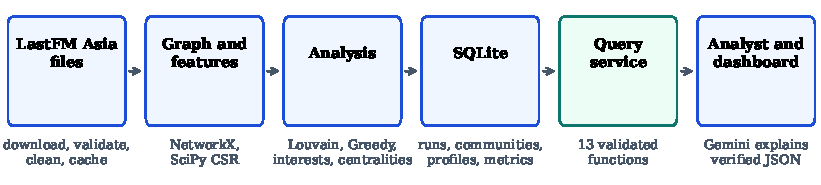
\includegraphics[width=0.95\textwidth]{figures/architecture.pdf}
\caption{Social DNA architecture. The LLM is the final stage and receives only verified JSON.}
\label{fig:arch}
\end{figure*}

\subsection{Graph construction and community detection}
Users are nodes and mutual follows are undirected edges of a NetworkX graph \cite{hagberg2008}; original dataset identifiers are used throughout. Self-loops, duplicate edges and edges to unknown users would be removed and counted. We use Louvain \cite{blondel2008} (python-louvain) with a configurable random seed and resolution (here seed 42, resolution 1) and greedy modularity optimisation \cite{clauset2004} as a deterministic comparison. Modularity for both is computed with the same NetworkX routine so the values are comparable. Communities are renumbered $1..k$ by decreasing size (ties broken by the smallest member identifier) so that a given grouping always receives the same numbers.

\subsection{Evaluation without ground truth}
Because no reference partition exists, we report (i) modularity, (ii) \emph{stability}: Louvain is run with 10 seeds and every pair of partitions is compared with NMI and ARI, and (iii) \emph{agreement} between Louvain and greedy modularity. These quantify consistency, not correctness, and we do not claim that either algorithm is more accurate.

\subsection{Interest profiling}
Let $X\in\{0,1\}^{n\times f}$ indicate which users like which artist features, and let $C$ be a community with $|C|$ members. For feature $j$ we define the frequency $\mathrm{fr}_j=\sum_{i\in C}X_{ij}$, the prevalence $p_j=\mathrm{fr}_j/|C|$, the network prevalence $q_j=\frac{1}{n}\sum_i X_{ij}$, and the lift $\ell_j=p_j/q_j$. The \emph{distinctiveness} of an over-represented feature ($\ell_j>1$) is
\begin{equation}
d_j = p_j\,\log_2 \ell_j ,
\end{equation}
where the factor $p_j$ prevents rare accidents from outranking widely shared features. Only features liked by at least $\max(3,\lceil 0.02|C|\rceil)$ members are eligible. \emph{Common} features are those with the highest frequency. All counts for all communities are obtained with one sparse matrix product.

\subsection{Similarity}
User vectors are weighted with a smoothed inverse document frequency $\mathrm{idf}_j=\ln\frac{1+n}{1+\mathrm{df}_j}+1$ and $L_2$-normalised, following TF-IDF practice \cite{salton1988}. A community profile is the mean of its members' vectors; communities are compared by cosine similarity. For unit vectors $u_i$ the mean pairwise cosine inside a community is exact and linear-time:
\begin{equation}
\bar{c}(C)=\frac{\left\lVert\sum_{i\in C}u_i\right\rVert^2-|C|}{|C|\,(|C|-1)} ,
\end{equation}
which we verify against brute force in the test suite. Jaccard similarity \cite{jaccard1901} between two communities is computed on their sets of the 30 most frequent features; within a community it is averaged over user pairs (sampled to 1{,}500 users for very large communities).

\subsection{Hubs and bridges}
We compute degree, closeness (exact), PageRank \cite{page1999} (exact) and betweenness \cite{freeman1977}. Exact betweenness is $O(nm)$, so we use sampled estimation \cite{brandes2007} with $k=1000$ source nodes and label it as an approximation wherever it is shown. For user $i$ with $k_i$ friends and $k_{ic}$ friends in community $c$, the participation coefficient is
\begin{equation}
P_i = 1-\sum_c \left(\frac{k_{ic}}{k_i}\right)^2 ,
\end{equation}
which is $0$ if all friends are in one community \cite{guimera2005}. A \emph{hub} has many friends; a \emph{bridge} is a user with degree $\ge 5$ and friends in at least three communities, ranked by betweenness.

\subsection{Verified LLM analyst}
The analyst answers questions in two steps. \emph{Routing:} Gemini \cite{gemini2023} is given 14 function declarations (13 analysis functions such as community details, common interests, comparison, bridge users, network report, and one \texttt{unsupported\_question} option) and is forced to call exactly one (function calling with temperature 0). If Gemini is unavailable a deterministic keyword router is used instead. \emph{Validation:} parameters are type-checked and community or user identifiers are validated against the stored results; invalid requests receive a corrective message and never reach the model. \emph{Explanation:} the function result, a JSON document built from the stored calculations, is passed to Gemini with a system prompt that forbids using any fact outside the data, forbids guessing artist names, and forbids claiming that one algorithm is more accurate. Questions the data cannot answer (weather, real identities, artist names, countries of communities) are refused. If the API is unreachable, the system shows a deterministic number-exact summary together with a notice; a short cool-down avoids waiting on every question during an outage. The model used was \texttt{gemini-3.5-flash-lite}, with fallback to other current Gemini models when one is overloaded or retired.

\section{Results}\label{sec:results}
\subsection{Communities}
Louvain finds 31 communities with modularity $Q=0.8155$. The largest community has 1025 users, the smallest 4, and the mean size is 246; the three largest hold 39.2\% of all users (Fig.~\ref{fig:sizes}). Only 8.1\% of friendships connect different communities.

\begin{figure}[t]
\centering
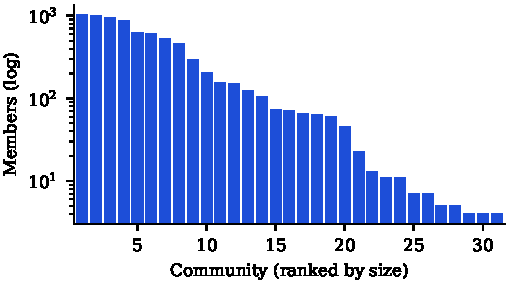
\includegraphics[width=0.95\columnwidth]{figures/sizes.pdf}
\caption{Community sizes (log scale), ranked. A few large communities coexist with a long tail of small ones.}
\label{fig:sizes}
\end{figure}

\subsection{Algorithm comparison and stability}
\begin{table}[t]
\caption{Louvain versus greedy modularity, and Louvain stability over 10 seeds}
\label{tab:algo}
\centering
\begin{tabular}{lr}
\toprule
Louvain: communities / modularity & 31 / 0.8155 \\
Greedy modularity: communities / modularity & 43 / 0.7960 \\
Louvain vs greedy: NMI / ARI (agreement) & 0.819 / 0.727 \\
Stability, mean pairwise NMI (min) & 0.900 (0.864) \\
Stability, mean pairwise ARI (min) & 0.877 (0.820) \\
Modularity over seeds (min--max, s.d.) & 0.8132--0.8162, 0.0009 \\
Communities over seeds (min--max) & 26--30 \\
\bottomrule
\end{tabular}
\end{table}

Table~\ref{tab:algo} shows that Louvain is stable: modularity varies by only about 0.003 across seeds although the number of communities varies between 26 and 30, which indicates that some fine-grained boundaries are seed-dependent while the coarse structure is not. Greedy modularity yields more communities (43) and slightly lower modularity (0.7960). Since both optimise the same objective, the modularity difference is not evidence that Louvain is more accurate, and there is no ground truth against which accuracy could be measured. For context only, the communities are strongly associated with the anonymised country code (NMI 0.624); this is consistent with homophily \cite{mcpherson2001} but is a descriptive association, not an accuracy score.

\subsection{Interests and similarity}
Community 1 (1025 members) is characterised by the features in Table~\ref{tab:feat}: the top distinctive feature is liked by about two thirds of its members but by under a fifth of all users. Inside communities the mean user-to-user cosine is only 0.123 (range 0.066--0.238) and mean pairwise Jaccard 0.096, i.e.\ friends share part of their taste but not most of it. Community profiles are much closer to each other: over the 465 community pairs the mean cosine is 0.448 (Fig.~\ref{fig:heat}); the most similar pair is communities 2 and 3 (cosine 0.880, Jaccard 0.395, 109 friendships between them) and the least similar pair has cosine 0.071.

\begin{table}[t]
\caption{Most distinctive artist features of community 1 (anonymous IDs)}
\label{tab:feat}
\centering
\begin{tabular}{rrrr}
\toprule
Feature ID & Community 1 & Whole network & Lift \\
\midrule
6576 & 64\% & 18\% & 3.5$\times$ \\
5417 & 62\% & 23\% & 2.7$\times$ \\
3501 & 53\% & 17\% & 3.1$\times$ \\
1763 & 54\% & 19\% & 2.9$\times$ \\
171 & 52\% & 18\% & 2.8$\times$ \\
\bottomrule
\end{tabular}
\end{table}

\begin{figure}[t]
\centering
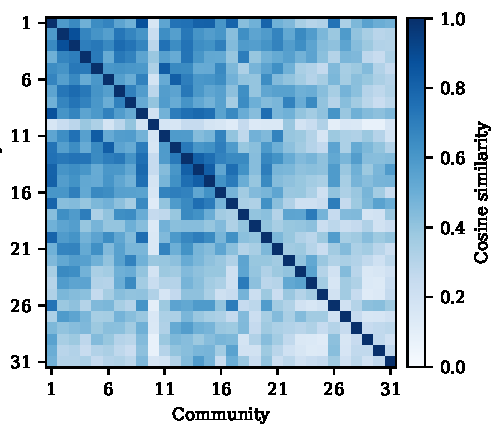
\includegraphics[width=0.9\columnwidth]{figures/heatmap.pdf}
\caption{Cosine similarity of TF-IDF interest profiles between all community pairs.}
\label{fig:heat}
\end{figure}

\subsection{Hubs and bridges}
\begin{table}[t]
\caption{A hub and a bridge (anonymised IDs; betweenness is sampled)}
\label{tab:hub}
\centering
\begin{tabular}{lrr}
\toprule
& Hub (user 7237) & Bridge (user 7199) \\
\midrule
Friends (degree) & 216 & 62 \\
Rank by degree & 1 & 56 \\
Friends outside own community & 13 & 37 \\
Communities reached & 8 & 13 \\
Participation coefficient & 0.116 & 0.789 \\
Betweenness (rank) & 0.0822 (2) & 0.0879 (1) \\
\bottomrule
\end{tabular}
\end{table}

Table~\ref{tab:hub} contrasts the user with the most friends with the highest-betweenness bridge. The hub has 216 friends but only 13 outside its own community, whereas the bridge has fewer friends (62, rank 56 by degree) but 37 of them outside its community, spread over 13 communities, and ranks 1 by betweenness. Both have similar betweenness values, yet they play different structural roles, which Fig.~\ref{fig:hub} shows is a general pattern: high participation appears at moderate degree. 570 users satisfy the bridge criterion.

\begin{figure}[t]
\centering
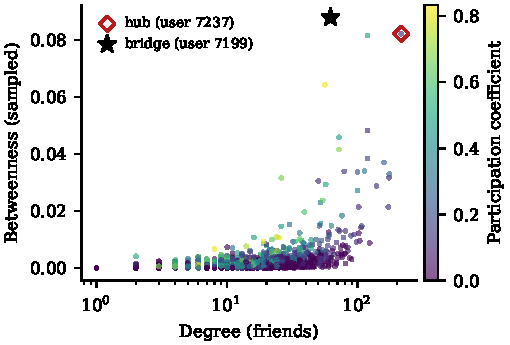
\includegraphics[width=0.95\columnwidth]{figures/hubbridge.pdf}
\caption{Degree versus sampled betweenness; colour shows the participation coefficient.}
\label{fig:hub}
\end{figure}

\subsection{Analyst evaluation}
\textbf{Protocol.} We use a fixed set of 29 questions: 23 answerable questions (network overview, community details, common interests, comparison, similarity, influential and bridge users, a user lookup, the Louvain explanation, the full report, and a follow-up that depends on the previous turn) and 6 questions the data cannot answer or that contain invalid parameters. Expected values are \emph{recomputed from the database} for each question and are never hard-coded. We measure: \emph{routing accuracy} (correct function and parameters); \emph{numerical correctness} (share of required key numbers found in the answer with precision-aware matching); \emph{unsupported-claim rate} (numbers in the answer that appear nowhere in the verified result; the structural numbers 1--5, 10 and 30 are ignored); \emph{missing-information handling} (refusal or correction without invented data); and a \emph{factual consistency} score, the per-answer mean of numerical correctness and one minus the unsupported share (1 or 0 for missing-information questions).

\textbf{Results.} Table~\ref{tab:eval} reports the deterministic router (no LLM), an initial live Gemini run, and the final live run. The final Gemini analyst reaches 95.7\% routing accuracy, 96.7\% numerical correctness, 0.1\% unsupported claims (1 of 769 numbers) and 95.1\% factual consistency; all five measures meet a 93\% target ($\le 7\%$ for the claim rate). Of the 23 answerable questions, 22 were answered by Gemini and 1 fell back to the deterministic summary after an API failure. The deterministic router scores 100\% by construction on its own templated answers (513 numbers checked), so it validates routing and the verified numbers, not the LLM's wording.

\begin{table}[t]
\caption{Analyst evaluation on 29 fixed questions}
\label{tab:eval}
\centering
\begin{tabular}{lrrr}
\toprule
Metric & Determ. & Gemini, run 1$^{*}$ & Gemini, final \\
\midrule
Routing accuracy & 100.0\% & 95.7\% & 95.7\% \\
Numerical correctness & 100.0\% & 88.8\% & 96.7\% \\
Unsupported-claim rate & 0.0\% & 0.3\% & 0.1\% \\
Missing-information handling & 100.0\% & 100.0\% & 100.0\% \\
Factual consistency & 100.0\% & 90.2\% & 95.1\% \\
\bottomrule
\end{tabular}

\vspace{2pt}
\footnotesize{$^{*}$Scored with the initial scorer (see text).}
\end{table}

\textbf{Scorer revision.} The first live run, scored with an initial scorer, gave numerical correctness 88.8\% and factual consistency 90.2\%, below the target. Inspection of the answers showed three scorer faults rather than model errors: a correct value 0.8155 was rejected because the scorer demanded the pre-rounded 0.815; questions such as ``how many communities'' were penalised for omitting facts they did not ask for; and ``anonymised'' was rejected because the check expected ``anonymous''. We corrected the scorer (precision-aware matching, per-question key facts, spelling tolerance), added regression tests, and re-ran the live evaluation. This revision was made after seeing the first run's answers, which is a form of post-hoc adjustment; we therefore report both runs. Genuine model misses remain counted against Gemini: for example, ``What do members of community 7 like?'' was routed to the community-details function instead of the interests function, and some answers omitted requested figures.

\textbf{Software verification.} The code base is covered by 76 automated tests on small synthetic graphs (used only for unit testing, never for reported results), including hand-computed modularity, brute-force checks of the similarity identities, persistence and constraint tests, invalid identifiers, missing API key, API failures, empty data, missing features, and tests showing that the evaluation scorer fails wrong answers.

\section{Discussion}\label{sec:disc}
\textbf{What the results mean.} The network is strongly modular ($Q=0.8155$) and only a small share of friendships cross communities, yet user-level taste similarity inside communities is modest. This suggests that friendship structure and shared taste are related but distinct, so describing a community by a single profile hides substantial within-group variety. The hub-versus-bridge contrast shows why degree alone is a poor proxy for a user's role in connecting groups.

\textbf{Why not report ``accuracy''.} Louvain is unsupervised and the dataset has no reference communities. Using the country code as a label would conflate geography with friendship communities; we report it only as a descriptive association. Modularity, stability and agreement measure internal consistency. A 93\% accuracy target is meaningful only for the analyst, where each answer can be checked against recomputed values.

\textbf{Threats to validity.} (i) The benchmark has only 29 questions, so one question changes a percentage by several points. (ii) Gemini is non-deterministic and results come from one run per scorer version. (iii) The scorer was revised after the first run, as disclosed. (iv) Numerical faithfulness does not prove that qualitative statements are correct. (v) Betweenness is an estimate from 1000 sampled sources.

\section{Limitations and Future Work}
The artist features are anonymous, so no artist names or genres can be reported. The data is a March 2020 snapshot of Asian users and the findings may not transfer. Louvain is heuristic and can yield badly connected communities \cite{traag2019}; the resolution limit \cite{fortunato2007} may hide small communities. Future work includes Leiden and overlapping community detection, a dataset with real artist names to enable semantic interest labels, temporal analysis of community change, and a larger, human-rated evaluation of explanation quality including qualitative claims.

\section{Conclusion}\label{sec:conc}
Social DNA demonstrates that community detection results can be explained in natural language without surrendering numerical integrity: calculations are performed by verified code, and the LLM only verbalises them. On LastFM Asia, Louvain finds 31 stable communities, interest profiling shows moderate internal and high cross-community similarity for specific pairs, and a grounded analyst answers questions with a very low unsupported-claim rate. We hope the explicit treatment of missing ground truth, honest reporting of a scorer revision, and fully reproducible code are useful for similar analyst tools.

\section*{Acknowledgment}
The authors thank the SNAP and FEATHER projects for releasing the LastFM Asia dataset. Source code, tests, evaluation results and the dashboard are available in the project repository ({[}repository URL{]}).

\begin{thebibliography}{00}
\bibitem{fortunato2010} S. Fortunato, ``Community detection in graphs,'' \emph{Phys. Rep.}, vol. 486, no. 3--5, pp. 75--174, 2010.
\bibitem{newman2006} M. E. J. Newman, ``Modularity and community structure in networks,'' \emph{Proc. Natl. Acad. Sci. USA}, vol. 103, no. 23, pp. 8577--8582, 2006.
\bibitem{blondel2008} V. D. Blondel, J.-L. Guillaume, R. Lambiotte, and E. Lefebvre, ``Fast unfolding of communities in large networks,'' \emph{J. Stat. Mech.}, vol. 2008, no. 10, P10008, 2008.
\bibitem{clauset2004} A. Clauset, M. E. J. Newman, and C. Moore, ``Finding community structure in very large networks,'' \emph{Phys. Rev. E}, vol. 70, no. 6, 066111, 2004.
\bibitem{traag2019} V. A. Traag, L. Waltman, and N. J. van Eck, ``From Louvain to Leiden: guaranteeing well-connected communities,'' \emph{Sci. Rep.}, vol. 9, art. 5233, 2019.
\bibitem{fortunato2007} S. Fortunato and M. Barth\'elemy, ``Resolution limit in community detection,'' \emph{Proc. Natl. Acad. Sci. USA}, vol. 104, no. 1, pp. 36--41, 2007.
\bibitem{danon2005} L. Danon, A. D\'iaz-Guilera, J. Duch, and A. Arenas, ``Comparing community structure identification,'' \emph{J. Stat. Mech.}, vol. 2005, no. 9, P09008, 2005.
\bibitem{hubert1985} L. Hubert and P. Arabie, ``Comparing partitions,'' \emph{J. Classif.}, vol. 2, no. 1, pp. 193--218, 1985.
\bibitem{bothorel2015} C. Bothorel, J. D. Cruz, M. Magnani, and B. Micenkov\'a, ``Clustering attributed graphs: models, measures and methods,'' \emph{Netw. Sci.}, vol. 3, no. 3, pp. 408--444, 2015.
\bibitem{mcpherson2001} M. McPherson, L. Smith-Lovin, and J. M. Cook, ``Birds of a feather: Homophily in social networks,'' \emph{Annu. Rev. Sociol.}, vol. 27, pp. 415--444, 2001.
\bibitem{salton1988} G. Salton and C. Buckley, ``Term-weighting approaches in automatic text retrieval,'' \emph{Inf. Process. Manag.}, vol. 24, no. 5, pp. 513--523, 1988.
\bibitem{jaccard1901} P. Jaccard, ``\'Etude comparative de la distribution florale dans une portion des Alpes et des Jura,'' \emph{Bull. Soc. Vaudoise Sci. Nat.}, vol. 37, pp. 547--579, 1901.
\bibitem{freeman1977} L. C. Freeman, ``A set of measures of centrality based on betweenness,'' \emph{Sociometry}, vol. 40, no. 1, pp. 35--41, 1977.
\bibitem{brandes2007} U. Brandes and C. Pich, ``Centrality estimation in large networks,'' \emph{Int. J. Bifurcation Chaos}, vol. 17, no. 7, pp. 2303--2318, 2007.
\bibitem{page1999} L. Page, S. Brin, R. Motwani, and T. Winograd, ``The PageRank citation ranking: Bringing order to the web,'' Stanford InfoLab, Tech. Rep., 1999.
\bibitem{guimera2005} R. Guimer\`a and L. A. N. Amaral, ``Functional cartography of complex metabolic networks,'' \emph{Nature}, vol. 433, pp. 895--900, 2005.
\bibitem{granovetter1973} M. S. Granovetter, ``The strength of weak ties,'' \emph{Am. J. Sociol.}, vol. 78, no. 6, pp. 1360--1380, 1973.
\bibitem{lewis2020} P. Lewis \emph{et al.}, ``Retrieval-augmented generation for knowledge-intensive NLP tasks,'' in \emph{Adv. Neural Inf. Process. Syst. (NeurIPS)}, vol. 33, 2020.
\bibitem{schick2023} T. Schick \emph{et al.}, ``Toolformer: Language models can teach themselves to use tools,'' in \emph{Adv. Neural Inf. Process. Syst. (NeurIPS)}, vol. 36, 2023.
\bibitem{ji2023} Z. Ji \emph{et al.}, ``Survey of hallucination in natural language generation,'' \emph{ACM Comput. Surv.}, vol. 55, no. 12, art. 248, 2023.
\bibitem{gemini2023} Gemini Team, Google, ``Gemini: A family of highly capable multimodal models,'' arXiv:2312.11805, 2023.
\bibitem{rozemberczki2020} B. Rozemberczki and R. Sarkar, ``Characteristic functions on graphs: Birds of a feather, from statistical descriptors to parametric models,'' in \emph{Proc. 29th ACM Int. Conf. Inf. Knowl. Manag. (CIKM)}, 2020, arXiv:2005.07959.
\bibitem{hagberg2008} A. A. Hagberg, D. A. Schult, and P. J. Swart, ``Exploring network structure, dynamics, and function using NetworkX,'' in \emph{Proc. 7th Python in Science Conf. (SciPy)}, 2008, pp. 11--15.
\end{thebibliography}

\end{document}
